\documentclass[a4paper, rebuttal, parskip=true, firsthead=false, fromemail=true, foldmarks=false]{scrlttr2}
\usepackage{amsmath}
\usepackage{amsfonts}
\usepackage{amssymb}
\usepackage{graphicx}
\usepackage[british]{babel}
%\address{Mathieu Leocmach and Hajime Tanaka,\\ Institute of Industrial Science,\\ University of Tokyo}
%\signature{Mathieu Leocmach and Hajime Tanaka} 
\begin{document} 
\begin{letter}{Dr. Nicky Dean\\
Associate Editor\\
Nature Communications}
\opening{\bf Dear Nicky,}

Thank you very much for your e-mail concerning our manuscript (NCOMMS\nobreakdash-12\nobreakdash-00580\nobreakdash-T) together with the comments of the Reviewers. 

We are delighted by your positive response and we revised our manuscript in order to comply with the format requirement of Nature Communications and the last suggestions of both Reviewers (see below for a detailed answer to each of your editorial requests). In particular, please note that we added two panels to the first figure of the main text: one comes from the former Supplementary Figure 3, which was suppressed; and the other is the data of the kurtosis of the displacement, asked by the Reviewer \#2. We hope you will agree that this purely formal change improves the readability of our paper. We also removed the section in Supplementary Methods about our first definition of the dynamical length. This was just a side note, not adding anything to our message and not cited anywhere in the main text.

We hope that you would find that the revised manuscript now fits the editorial standards for publication in Nature Communications.

\closing{\bf Sincerely yours,} 
\clearpage

\textsf{\textbf{Replies to the confidential comments of Reviewer \#2}}

\begin{quotationi}
In their confidential comments to the editor, Reviewer \#2 suggests that the scientific context for the work needs to be better explained, in order to make the results understood more clearly within the surrounding field. This is based on their understanding that the particular system studied here is one in which one of the length scales and the dynamical length scale grow together. This is in contrast to other works that show very different behaviour (e.g. Kob et al., Nature Physics 8, 164 (2012); Charbonneau et al., Phys. Rev. Lett. 108, 035701 (2012)). Reviewer \#2 suggests that the results in your manuscript could be fortuitous to the particular system studied or it may represent a class of different systems where a connection between these length scales does exist, which may then be an echo of coupling in two-dimensional glass forming liquids. Based on this advice, we feel it would be appropriate to modify the introduction to provide more of this view, giving better context for the new findings in relation to ongoing efforts. To aid in this, Reviewer \#2 provided us with the following three additional comments:
\begin{itemize}
\item The presentation of the theoretical and simulation context should be improved. In particular, the theoretical importance of the dynamical and the static length scales, which is a corner stone of the debate between geometrical frustration-based descriptions, facilitation-based descriptions, and the RFOT theory, should be better discussed.

\item Although a static length scale was proven to grow with relaxation time by Montanari and Semerjian (Journal of Statistical Physics DOI: \\ 10.1007/s10955\nobreakdash-006\nobreakdash-9175\nobreakdash-y), the physical relevance of that length scale may vary with the specific relaxation regime considered and/or the type of glassy dynamics. Two recent studies have shown that the two types of length scales (static \& dynamical) can have very different behavior as the system becomes sluggish. Charbonneau, Charbonneau, and Tarjus (Physical Review Letters, DOI: 10.1103/PhysRevLett.108.035701) have shown that the growth of the two lengths can be decoupled, which is in agreement with both a facilitation-based description and RFOT theory, but not geometrical frustration; while Kob, Roldán-Vargas and Berthier (Nature Physics, DOI: 10.1038/NPHYS2133) have shown that the dynamical length can behave non-monotonically as the static length steadily grows, which is reminiscent of a critical-like behavior and is only consistent with
RFOT theory.
\end{itemize}
\end{quotationi}

We tried to better explain the context of our work in the light of the confidential comment of Reviewer \#2. We cited the recent simulation results of Kob et al. as well as the theoretical results of Montanari and Semerjian. We are aware of the contradictions between the results obtained by Charbonneau et al. and the class of systems studied here and in our previous papers. Thus we reformulated some of our statements that may have appeared too general to the Reviewer, restricting them to `a class of system'.

\begin{quotationi}
\begin{itemize}
\item The system studied by the authors exhibits a qualitatively different behavior. Both static and dynamical length scales grow together, which may indicate that the system is part of a class for which geometrical frustration or a related description is more appropriate. This family of systems could be the three-dimensional equivalent of what is observed in many two-dimensional systems. A possible connection between this subset of two- and three-dimensional systems may be the relative similarity between the local liquid and the crystal orders, as observed here. In 2d this similarity is quite common, but in 3d the similarity may be quite sensitive to the particle size distribution present. For other size distributions, such as that studied by Charbonneau et al. for instance, such similarity is indeed not observed. Van Meel et al. (Physical Review E DOI: 10.1103/PhysRevE.80.061110) have further shown that in higher dimensions the similarity between liquid and crystal order rapidly vanishes, although these systems remain exhibit the typical glass forming phenomenology (Physical Review E DOI: 10.1103/PhysRevE.81.040501).
\end{itemize}
\end{quotationi}

Reviewer \#2 suggests a link between our family of systems and two-dimensional ones, as opposed to other three-dimensional systems rather linked to four-dimensional case. We think this point is speculative and we see nothing in our data either for or against it. Thus we prefer to stand by our general statement in the Discussion that ``the generality and limitation of [our] scenario need to be checked carefully in the future''.

\textsf{\textbf{Replies to editorial requests}}

\begin{quotationi}
* The abstract must be less than 150 words and may not contain references.
\end{quotationi}
We removed the references in the abstract which is below 150 words.

\begin{quotationi}
* In the Introduction, the results and conclusions of the paper should only be discussed in the final paragraph. Please merge the last two paragraphs to meet this requirement.
\end{quotationi}
We merged the two paragraphs.

\begin{quotationi}
* Please carefully check the language of the paper; perhaps a colleague who is a native English speaker could check over it. There are some errors, such as:
- "The nature of the glass transition (thermodynamic or kinetic, structural or purely dynamical) is still [a] matter of [debate]..."
- "We will show that both [kinds] of disorder are..."
- "([dodecahedra] are present but can be considered as twisted [icosahedra])"
- "Both types of packing have low local free energy and thus [are] locally favoured"
\end{quotationi}
Thank you for your careful reading. We corrected the errors you pointed and we asked for more proof reading around us.

\begin{quotationi}
* Please note that our style does not allow for the use of italic emphasis. Please remove this wherever it is used.
\end{quotationi}
We removed all italic emphasis.

\begin{quotationi}
* Mathematical subscripts and superscripts should only be italic for variables. Abbreviations ("dod", "max" etc) should not be italic.
\end{quotationi}
The mathematical subscript and superscript are now in Roman font.

\begin{quotationi}
* The Methods section should be no more than 1500 words. Please reduce the number of words to within this limit. Language can be more concise here.
\end{quotationi}
We reduced the number of words in Methods below 1500 words. A few sentences were transferred from the Methods/Dynamic to the Results/Dynamics.

\textsf{References}
\begin{quotationi}
* Please ensure all references are formatted in the Nature style. Reference 39 is missing a journal title and volume.
\end{quotationi}
Reference 39 was a preprint, thus going against the publication guidelines of Nature Communications. We removed it.

\textsf{Figures}
\begin{quotationi}
* Please supply figures so that every element of each figure is editable (i.e. we can highlight and edit the text, and move individual parts of the figures around). When making these changes please ensure resolution stays high at 300dpi.
\end{quotationi}

Our figures are in a vectorial editable format and will be sent as PDF. Bitmap pictures included and in high resolution, except for the bond-order population maps where the pixel size is the bin size of our histogram and are thus at highest possible resolution.

\begin{quotationi}
* Ensure all figures are cited in order in the text. Figures 4 and 5 are cited out of sequence.
\end{quotationi}
We fixed the citation order of our figures. They are now cited in order in the text.

\begin{quotationi}
* Remove boxes from around plots, leaving only x and y axes.

* Each x- and y-axis should be individually labelled. Please separate panels and provide axis labels where needed.

* Figures appear at 9 or 18 cm width - 1 or 2 columns respectively.

* Please supply units for axis titles.
\end{quotationi}
We removed boxes from around plots, separated the axis and provided the needed labels. All our figures are meant to appear on two columns and are designed accordingly. We supplied units everywhere we plotted non-dimensionless values.

\begin{quotationi}
* Figure 1. Please separate a and b and reduce figure clutter by removing the keys in panel b and explaining the symbols in the caption.
\end{quotationi}
We separated all the panels and removed the key to reduce figure clutter. We also added two panels: b requested by Referee \#2 and c from a previous Supplementary figure. We colour-coded the five samples coherently in a,b,c so that a single key is needed.

\begin{quotationi}
* Figure 2. The caption is confusing. The second sentence "For our deepest..." does not make sense by itself. It should be rewritten so that it is clear what this means. Is it possible to make all the panels the same size so that the layout appears more ordered? All lines on the plots should be explained in the caption, including the horizontal and vertical lines through the axes.
\end{quotationi}
We reformulated the caption and explained the horizontal and vertical lines. We reworked the layout so that the panels are aligned and of the same size. We hope you will find it more ordered.

\begin{quotationi}
* Figure 3. Please explain the vertical and horizontal lines in panel a. To reduce figure clutter, please remove the phi label in the upper left corner and put this information in the caption. Separate panels b and c and provide y axis titles for both panels. The vertical and horizontal lines should be explained in the caption. To reduce figure clutter and improve the readability of the panels, it would be better to remove the key to symbols and phi in panel c and explain them in the caption instead.
\end{quotationi}
We explained straight lines in (a-c) and reduced figure clutter. Colour code for the samples is now the same as in Figure 1.

\begin{quotationi}
* Figure 4. To improve the readability of the data, please remove the grid lines and any unnecessary framing lines. Please do not refer the reader to the text for details. Any information important to the caption should be given there.
\end{quotationi}
We removed grid and framing lines and made the caption self-consistent.


\begin{quotationi}
* Figure 5. In panel, please remove the label "$w_6<-0.012$" as this is already given in the caption. Please describe the straight line in the caption. In panel b, please explain the straight lines and labels, removing any that can be given in the caption instead. In panel d, please explain the vertical lines. In panel d, please remove the key to symbols and ensure this is adequately explained in the caption.
\end{quotationi}
We remove labels on the figure and used the caption to explain.

\textsf{Supplementary Information}
\begin{quotationi}

* The Supplementary Information should contain subheaded sections. Permitted subheadings are: Supplementary Methods, Supplementary Discussion, Supplementary Figure, Supplementary Table, and Supplementary References. The text in the Supplementary Information should be placed under the heading of Supplementary Methods. The Supplementary Information should then be ordered in the following way: Supplementary Figures, Supplementary Methods, and Supplementary References. Supplementary Figures should appear with their captions on the same page; captions should not overrun onto separate pages.
\end{quotationi}
We reorganized our Supplementary Information to have the Supplementary Figures coming first.

\begin{quotationi}
* Supplementary References should be numbered following on from the main text, so in this case beginning at 54. They should be formatted in the same style as the main paper.
\end{quotationi}
Supplementary References now follows main text's numbering. We removed one of the references that was a preprint.


\begin{quotationi}
* In the main paper, please do not cite 'Supplementary Information'. Instead, please refer to specific items of the Supplementary Information (Supplementary Figure SX, Supplementary Methods). All items must be cited, and Supplementary Figures must be cited in order.
\end{quotationi}

We now cite Supplementary Methods. The sub-part of Supplementary Method that was not cited in the main text (about $G_u$ and $\xi_u$) was removed. Remaining Supplementary Figures are cited in order.

\begin{quotationi}
* Supplementary Figures should be labelled and referred to as Supplementary Figure S1, not Fig S1, throughout both the Supplementary Information and the main text.
\end{quotationi}
We checked that point.


\textsf{Miscellaneous}
\begin{quotationi}

* Please provide us with an image to use as a thumbnail on our website. Please see the attached sheet for formatting information.

* Please consider whether you could provide us with an arresting image to use as a featured image on our website.
\end{quotationi}

\includegraphics{thumbnail.jpg}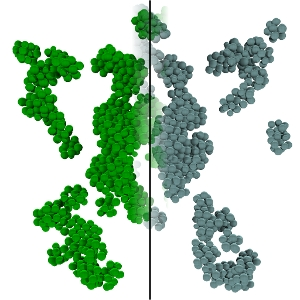
\includegraphics{cover.jpg}

We provide both pictures. The text corresponding to the featured image should include somthing like ``Two sides of the same coin: Dynamical heterogeneities (right) reflect large scale structural heterogeneities (left). Right panel was flipped.''

\begin{quotationi}
* Your article will be accompanied by a short, accessible editor's summary on our homepage. I propose:

"The dynamics and structure of the glass transition in liquids is still debated. Using particle-level confocal microscopy, Leocmach and Tanaka investigate supercooled colloidal liquids and distinguish different scenarios for the glass transition, suggesting that local ordering may only play a minor role."

Please let me know if this is inaccurate or if you would like to suggest improvements (there is a 310 character limit, including spaces).
\end{quotationi}
This summary fits, provided the character limit. However it may confuse the reader, especially if our featured image represents crystal-like order fitting the pattern of dynamical heterogeneities. Maybe adding ``\textit{very} local order'' would induce less confusion. Or ``suggesting that only medium range ordering may play a role.''

\clearpage
\textbf{Replies to the comments of Reviewer \#2}

First, we thank the Reviewer for his or her valuable comments since the beginning of this review process.

\begin{quotationi}
The manuscript is now more reasonable, although a couple of small things are still missing.

- On p. 3 4th line, the authors probably (really) mean to write "Modern spin-glass-type theories" or "Modern spin-glass-like theories". The structural glasses are not spin glasses, although an analogy has been drawn by some.
\end{quotationi}
We fixed this language abuse.

\begin{quotationi}
- In Fig. 1, the wave vector at which $\tau_\alpha$ is extracted should be reported. If the cutoff function $w_i(t)$ is used, it should also be mentioned.
\end{quotationi}
We indicated the wave vector in the caption of Fig.~1.

\begin{quotationi}
- The results for the kurtosis of the displacements $\alpha_2(t)$ (Eq. 1), which are discussed in the text, should be included in the SI.
\end{quotationi}

We included a panel in Fig.~1 to plot our $\alpha_2(t)$ results. We also moved the second (and most informative) panel of former Supplementary Figure 3 to Fig.~1. Former Supplementary Figure 3 was suppressed (the two panels were redundant).

We hope that the Reviewer would think that the revised manuscript is now suitable for publication in Nature Communications. 

\clearpage
\textbf{Replies to the comments of Reviewer \#3}
\begin{quotationi}
I'm happy with the revised manuscript, the supplemental materials are now clear.
\end{quotationi}

We thank the Reviewer for his or her valuable comments since the beginning of this review process.

\end{letter} 
\end{document}